\documentclass[11pt,a4paper]{article}
\usepackage[spanish,es-nodecimaldot]{babel}	% Utilizar español
\usepackage[utf8]{inputenc}					% Caracteres UTF-8
\usepackage{graphicx}						% Imagenes
\usepackage[hidelinks]{hyperref}			% Poner enlaces sin marcarlos en rojo
\usepackage{fancyhdr}						% Modificar encabezados y pies de pagina
\usepackage{float}							% Insertar figuras
\usepackage[textwidth=390pt]{geometry}		% Anchura de la pagina
\usepackage[nottoc]{tocbibind}				% Referencias (no incluir num pagina indice en Indice)
\usepackage{enumitem}						% Permitir enumerate con distintos simbolos
\usepackage[T1]{fontenc}					% Usar textsc en sections
\usepackage{amsmath}						% Símbolos matemáticos

\usepackage{listings}
\usepackage[dvipsnames]{xcolor}

\definecolor{codegreen}{rgb}{0,0.6,0}
\definecolor{codegray}{rgb}{0.5,0.5,0.5}
\definecolor{codepurple}{rgb}{0.58,0,0.82}
\definecolor{backcolour}{rgb}{0.95,0.95,0.92}

\lstdefinestyle{mystyle}{
    backgroundcolor=\color{backcolour},   
    commentstyle=\color{codegreen},
    keywordstyle=\color{magenta},
    numberstyle=\tiny\color{codegray},
    stringstyle=\color{codepurple},
    basicstyle=\ttfamily\footnotesize,
    breakatwhitespace=false,         
    breaklines=true,                 
    captionpos=b,                    
    keepspaces=true,                 
    numbers=left,                    
    numbersep=5pt,                  
    showspaces=false,                
    showstringspaces=false,
    showtabs=false,                  
    tabsize=4,
    language=C++
}

\lstset{style=mystyle}

% Comando para poner el nombre de la asignatura
\newcommand{\asignatura}{Arquitectura y Computación de Altas Prestaciones}
\newcommand{\autor}{Vladislav Nikolov Vasilev}
\newcommand{\titulo}{Práctica 5}
\newcommand{\subtitulo}{Paralelización del filtro de mediana mediante CUDA}
\newcommand{\rama}{Ingeniería de Computadores}

% Configuracion de encabezados y pies de pagina
\pagestyle{fancy}
\lhead{\autor{}}
\rhead{\asignatura{}}
\lfoot{Grado en Ingeniería Informática}
\cfoot{}
\rfoot{\thepage}
\renewcommand{\headrulewidth}{0.4pt}		% Linea cabeza de pagina
\renewcommand{\footrulewidth}{0.4pt}		% Linea pie de pagina

\begin{document}
\pagenumbering{gobble}

% Pagina de titulo
\begin{titlepage}

\begin{minipage}{\textwidth}

\centering

%
\includegraphics[scale=0.5]{img/ugr.png}\\

\includegraphics[scale=0.3]{img/logo_ugr.jpg}\\[1cm]

\textsc{\Large \asignatura{}\\[0.2cm]}
\textsc{GRADO EN INGENIERÍA INFORMÁTICA}\\[1cm]

\noindent\rule[-1ex]{\textwidth}{1pt}\\[1.5ex]
\textsc{{\Huge \titulo\\[0.5ex]}}
\textsc{{\Large \subtitulo\\}}
\noindent\rule[-1ex]{\textwidth}{2pt}\\[3.5ex]

\end{minipage}

%\vspace{0.5cm}
\vspace{0.7cm}

\begin{minipage}{\textwidth}

\centering

\textbf{Autor}\\ {\autor{}}\\[2.5ex]
\textbf{Rama}\\ {\rama}\\[2.5ex]
\vspace{0.3cm}


\includegraphics[scale=0.3]{img/etsiit.jpeg}

\vspace{0.7cm}
\textsc{Escuela Técnica Superior de Ingenierías Informática y de Telecomunicación}\\
\vspace{1cm}
\textsc{Curso 2019-2020}
\end{minipage}
\end{titlepage}

\pagenumbering{arabic}
\tableofcontents
\thispagestyle{empty}				% No usar estilo en la pagina de indice

\newpage

\setlength{\parskip}{1em}

\section{Introducción}

El objetivo de esta práctica es paralelizar, mediante \texttt{CUDA}, un algoritmo secuencial que
trabaje con estructuras de datos 2D tales como podrían ser matrices. Una vez que se ha
paralelizado, se tienen que tomar medidas de los tiempos y obtener la ganancia según la
cantidad de trabajo que tenga que hacer cada hebra (granularidad). Los tiempos
obtenidos se compararán con los de la versión secuencial y la versión en \texttt{MPI}, la cuál
fue implementada anteriormente. Este estudio se tiene que hacer con dos problemas de tamaño
diferente, uno más pequeño y uno más grande.

\section{Algoritmo escogido: filtro de mediana}

El algoritmo que se ha escogido paralelizar es el \textbf{filtro de mediana}. Este es un
filtro bastante sencillo y utilizado en el procesamiento de imágenes ya que permite eliminar
el \textbf{ruido sal y pimienta} de estas. Este tipo de ruido se caracteriza por la presencia
de píxeles blancos y negros en la toda la imagen, los cuáles son producto de alguna perturbación
de la señal de la imagen. Un ejemplo se puede ver a continuación:

\begin{figure}[H]
    \centering
    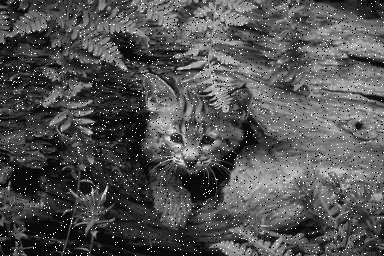
\includegraphics[scale=0.6]{img/cat.png}
    \caption{Imagen con ruido sal y pimienta.}
    \label{fig:cat}
\end{figure}

El algoritmo consiste en iterar sobre los píxeles de la imagen, coger una región de tamaño
$k \times k$ píxeles alrededor del actual (donde $k$ es el tamaño del filtro), ordenar
los valores y escoger el valor mediano, el cuál será el píxel de salida. Un ejemplo de este
procedimiento se puede ver a continuación:

\begin{figure}[H]
  \centering
  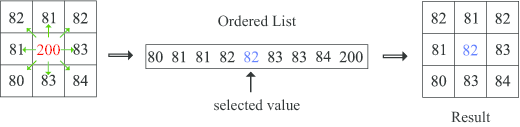
\includegraphics[scale=0.4]{img/median-filter.png}
  \caption{Ejemplo del filtro de mediana.}
  \label{fig:median-filter}
\end{figure}

Si aplicamos este filtro a la figura \ref{fig:cat}, obtendríamos el siguiente resultado:

\begin{figure}[H]
  \centering
  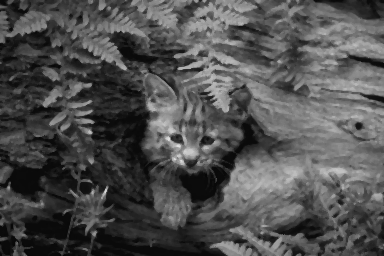
\includegraphics[scale=0.6]{img/filtered-cat}
  \caption{Imagen a la que se le ha aplicado el filtro de mediana.}
  \label{fig:filtered-cat}
\end{figure}

\section{Paralelización}

Ya que la versión secuencial fue explicada anteriormente, vamos a pasar a hablar directamente
de la paralelización que se ha realizado. En este caso, la paralelización es diferente a la que
se hacía en \texttt{MPI}, ya que siguen filosofías diferentes.

Se parte de una imagen de tamaño $w \times h$, donde $w$ es la anchura y $h$ la altura. La
imagen de salida tiene el mismo tamaño, pero recordemos que para poder aplicar el filtro se
tienen que replicar los bordes la imagen. Esto se hace para que el filtro se pueda aplicar de
igual manera por toda la imagen original, incluso por los bordes, donde en un principio, si
no se replicasen los bordes, se tendrían menos píxels, lo cuál obligaría a hacer un filtro
adaptativo al entorno del píxel. Esto sería contraproducente, ya que implicaría introducir
bloques condicionales en el \textit{kernel}, y al ejecutar todas las hebras el mismo código,
se ejecutaría dicho bloque de manera casi secuencial.

Esta replicación se hace al cargar la imagen, con lo cuál el \textit{kernel} no se tiene que
preocupar por eso. Recordemos que al replicar los bordes, la imagen sobre la que se aplica el
filtro es algo como lo que se puede ver a continuación:

\begin{figure}[H]
  \centering
  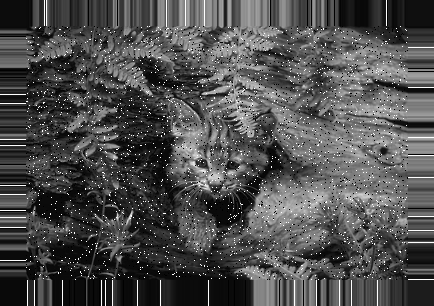
\includegraphics[scale=0.6]{img/borders-cat}
  \caption{Ejemplo de la replicación de bordes con filtro de tamaño $k = 101$.}
  \label{fig:borders-cat}
\end{figure}

Ya que estamos trabajando con una estructura de datos 2D como es una imagen, lo lógico es
crear un \textit{grid} 2D donde cada bloque esté indexado por una pareja $(x, y)$, donde $x$
es el índice en la dimensión $X$ e $y$ el índice en la dimensión $Y$. Cada bloque se
encargará de generar una región de $n \times n$ píxeles de la imagen de salida.
Se tiene por tanto que el \textit{grid} tiene un tamaño de $\frac{w}{n} \times \frac{h}{n}$
bloques. Para asegurar un reparto correcto, lo mejor es trabajar con imágenes cuya anchura y
altura sean potencias de 2, además de que el valor de $n$ también tiene que ser una potencia
de 2. De esta forma, no habrá bloques que generen regiones que se salgan de los límites de la
imagen, por ejemplo.

Aparte de esto, se tiene que los bloques también son bidimensionales, de manera que cada región
de la imagen de salida es generada de forma más fácil. Esto significa que se tiene \textbf{un
\textit{grid} 2D de bloques 2D}.

En cada bloque, cada hebra estará identificada por una pareja $(x_t, y_t)$, donde $x_t$ es el
índice en la dimensión $X$ del bloque e $y_t$ es el índice en la dimensión $Y$ del bloque.
Cada hebra se encargará de procesar una región dentro del bloque de $m \times m$ píxeles.
Cuanto menor sea el valor de $m$, se tendrá una granularidad más fina, mientras que a mayor
valor se tendrá una granularidad más gruesa, ya que cada hebra hará más trabajo. En un bloque
habrán $\frac{n}{m} \times \frac{n}{m}$ hebras, de manera que a menor valor, habrán más hebras,
mientras que a mayor valor, menos. Al ser $n$ una potencia de 2, para asegurar un reparto
correcto $m$ tendría que ser una potencia de 2 también, de manera que el reparto de trabajo
sea equitativo.

Para poder aplicar el filtro correctamente en cada bloque y generar una región de $n \times n$
píxeles hacen falta píxeles de los bloques vecinos, y de los bordes en el caso de que el bloque
esté en un extremo. Esto, por tanto, implica que cada bloque debe tener algo como una
\textbf{ventana local}, la cuál va a contener los píxels a utilizar. El tamaño de esta ventana
es de $l \times l$ píxeles, donde $l$ viene dado por:

\begin{equation}
l = n + 2 \cdot b
\end{equation}

\noindent donde $b$ es el tamaño del borde, el cuál es el resultado de la división entera
$\lfloor \frac{k}{2} \rfloor$.

Es de suma importancia destacar un aspecto muy importante, y es que, a pesar de que una
imagen se pueda representar como un \textit{array} 2D, tenemos que transformar dicho
\textit{array} a uno 1D. Esto se debe a que las funciones de reserva de memoria de
\texttt{CUDA} reservan memoria en posiciones contiguas, y es mucho más fácil hacer esto para
\textit{arrays} 1D que para los 2D. Por tanto, en vez de tener una estructura 2D con $h$ filas
y $w$ columnas, tendremos un \textit{array} 1D de tamaño $h \times w$. De la posición $0$ a
la $w-1$ irá la primera fila, de la $w$ a la $2w - 1$ la segunda, y así consecutivamente hasta
llegar a la última fila, la cuál irá desde la posición $(h-1)w$ hasta la $hw - 1$.

Una vez que hemos hablado de cómo se hace la división de la imagen en bloques y hebras y de
cómo se representan las imágenes, vamos a ver cómo se ha implementado el \textit{kernel} y lo
vamos a ir comentando. Dicho \textit{kernel} puede encontrarse en el fichero
\texttt{medianKernel.cu}, y a continuación se muestra dicho código:

\begin{lstlisting}
__global__ void medianKernel(float* dSrc, float* dDest,
							 int srcWidth, int destWidth,
							 int kernelSize, int windowSize,
							 int expandedWindowSize,
							 int pixelsPerThread)
{
    // Window which contains all the pixels that will be used in this block
    extern __shared__ float localWindow[];

    int xStartBlock = blockIdx.x * windowSize;
    int yStartBlock = blockIdx.y * windowSize;

    int xIdx = threadIdx.x;
    int yIdx = threadIdx.y;

    int xStartWindow = xIdx * pixelsPerThread;
    int yStartWindow = yIdx * pixelsPerThread;

    // Load local window from global memory and store it in local memory
    for (int j = yIdx; j < expandedWindowSize; j += blockDim.y)
    {
        for (int i = xIdx; i < expandedWindowSize; i += blockDim.x)
        {
            localWindow[j*expandedWindowSize + i] = dSrc[
            (yStartBlock + j) * srcWidth + xStartBlock + i];

        }
    }

    // Wait for all threads in the block to finish loading the data
    __syncthreads();

    // Allocate memory for kernel
    int kernelSquareSize = kernelSize * kernelSize;
    float* kernel = new float[kernelSquareSize];

    // Process local region inside local window
    for (int j = 0; j < pixelsPerThread; j++)
    {
        for (int i = 0; i < pixelsPerThread; i++)
        {
            // Get kernel's values
            for (int y = 0; y < kernelSize; y++)
            {
                for (int x = 0; x < kernelSize; x++)
                {
                    kernel[y*kernelSize + x] =
                    localWindow[(yStartWindow + j + y) * 
                       expandedWindowSize + xStartWindow + i + x];
                }
            }

            // Sort values and get median
            thrust::sort(thrust::seq, kernel,
            	kernel + kernelSquareSize);
            float median = kernel[kernelSquareSize / 2];
            dDest[(yStartBlock + yStartWindow + j) * destWidth +
            	xStartBlock + xStartWindow + i] = median;
        }
    }

    // Free memory
    delete[] kernel;
}
\end{lstlisting}

En la línea 8 se declara un \textit{array} dinámico compartido por todas las hebras de
un bloque. Esta es la manera de declararlo, y más adelante veremos cómo se hace la reserva
de memoria, la cuál se hace antes de la llamada al \textit{kernel}. Este \textit{array}
contendrá la \textbf{ventana local} de la que se habló anteriormente, es decir, todos los píxeles
que se van a necesitar para producir la región de salida. Al tener dicha información
en memoria local, los accesos posteriores van a ser más rápidos que si se quisiera acceder
a memoria global.

Una vez hecho esto se obtienen las posiciones de inicio del bloque (líneas 10-11). Se
multiplican los índices por el \textit{tamaño de ventana} o tamaño de bloque (a lo que
anteriormente habíamos llamado $n$). Los valores obtenidos hacen referencia son coordenadas
2D, pero más adelante se harán las transformaciones necesarias para que el acceso sea al
\textit{array} 1D. Se obtienen también los índices de las hebras y los índices de inicio en
la ventana/bloque (líneas 16-17). Estos últimos índices dependen de la granularidad (variable
\texttt{pixelsPerThread}).

Una vez hecho esto, en las líneas 20-28 se puede ver un doble bulce anidado. Su funcionalidad
es acceder a memoria global y copiar los píxeles necesarios para rellenar la
\textbf{ventana local}. El trabajo se reparte entre todas las hebras del bloque, de manera
que todas participen a la hora de traer los datos.

Una vez que la hebra ha terminado de copiar los datos que le correspondían tiene que esperar a
que todas terminen, ya que antes de continuar la \textbf{ventana local} tiene que tener
todos los datos. Esto se debe a que puede que haya alguna hebra que todavía no haya terminado
de copiar su parte y que otra hebra necesite acceder a esa información, con lo cuál se produciría
un error, ya que la información no está disponible todavía. Para ello, en la línea 31 se ha
introducido una llamada a una función de sincronización. De esta manera, hasta que todas las
hebras no hayan ejecutado esa función, no se podrá continuar con la ejecución del
\textit{kernel}.

En las líneas 34-35 se declara el \textit{kernel}, el cuál es un \textit{array} dinámico
1D local a cada hebra. Es en este \textit{array} donde se irán poniendo los valores del filtro
para posteriormente ordenarlos y obtener la mediana, el cuál será el píxel de salida.

En las líneas 38-60 se pueden ver cuatro bucles anidados. Los dos primeros bucles están
asociados a la granularidad. Es decir, hacen referencia a la región de tamaño $m \times m$ que
tiene que rellenar cada hebra dentro de la ventana/bloque, tal y como comentamos antes.
Los dos bulces internos (líneas 43-51) son los encargados de rellenar el \textit{kernel}
a partir de la \textbf{ventana local} para un píxel dado. Una vez que el \textit{kernel} está
relleno, se le aplica un algoritmo de ordenación (llamada a la función \texttt{thrust::sort()}).
Esta función ya está implementada dentro de las bibliotecas \texttt{CUDA}, y para que
pueda ser ejecutada por una hebra debe indicarse que la política (primer parámetro)
es secuencial mediante el valor \texttt{thrust::seq}. Una vez que el \textit{kernel} está
ordenado, se obtiene la mediana y posteriormente se asigna al correspondiente píxel de salida.

Finalmente, pero no por ello menos importante, una vez que la hebra ha terminado de procesar
su región $m \times m$ se tiene que liberar la memoria reservada para el \textit{kernel}
(línea 63).

Para poder exponer el \textit{kernel} al programa principal se ha creado un \textit{wrapper}
mediante una función normal de \texttt{C++}. Se ha hecho así para evitar problemas a la hora
de compilar el código. Esta función se puede ver a continuación:

\begin{lstlisting}
float* medianFilter(float* hSrc, int width, int height,
					int kernelSize, int windowSize,
					int pixelsPerThread, double& execTime)
{
    // Size of image with replicated borders
    int borderSize = kernelSize / 2;
    int srcWidth = width + 2*borderSize;
    int srcHeight = height + 2*borderSize;

    // Allocate local memory for filtered image
    float* hDest = new float[width * height];

    // Allocate memory for images in devide
    float* dSrc;
    float* dDest;

    cudaMalloc(&dSrc, srcWidth * srcHeight * sizeof(float));
    cudaMalloc(&dDest, width * height  * sizeof(float));

    // Define grid and block sizes
    dim3 gridSize((width - 1) / windowSize + 1, (height - 1) / windowSize + 1, 1);
    dim3 blockSize(windowSize / pixelsPerThread, windowSize / pixelsPerThread, 1);

    // Compute size of shared memory (in Bytes)
    int expandedWindowSize = windowSize + borderSize * 2;
    int sharedMemory = expandedWindowSize * expandedWindowSize * sizeof(float);

    auto t1 = std::chrono::high_resolution_clock::now();

    // Copy image to device
    cudaMemcpy(dSrc, hSrc, srcWidth * srcHeight * sizeof(float),
    	cudaMemcpyHostToDevice);


    // Apply median filter by calling the kernel
    medianKernel<<<gridSize, blockSize, sharedMemory>>>(dSrc,
    	dDest, srcWidth, width, kernelSize, windowSize, 
    	expandedWindowSize, pixelsPerThread);

    // Copy result from device
    cudaMemcpy(hDest, dDest, width * height * sizeof(float),
    	cudaMemcpyDeviceToHost);


    auto t2 = std::chrono::high_resolution_clock::now();
    execTime = std::chrono::duration<double>(t2 - t1).count();

    // Free device memory
    cudaFree(dSrc);
    cudaFree(dDest);

    return hDest;
}
\end{lstlisting}

Lo primero que hace es calcular el tamaño del borde (a lo que llamamos $b$ anteriormente)
en la línea 6. En las líneas 7-8 se determina la anchura y altura de la imagen fuente (aquella
imagen que tiene los bordes replicados). Después, en la línea 11 se reserva memoria para la
imagen resultado en el \textit{host}. En las líneas 14-18 se declaran los \textit{arrays} que
estarán en el dispositivo y se reserva la memoria para ellos. En la línea 21 se declara
el tamaño del \textit{grid}, el cuál puede verse que será 2D. Posteriormente, en la línea
22 se declara el tamaño del bloque. Una vez hecho esto, en la línea 25 se calcula el tamaño
de la \textbf{ventana local} y en la 26 se calcula el tamaño de dicha ventana en bytes (se
reservará tanta memoria posteriormente). Se procede luego a copiar la imagen fuente al
dispositivo (líneas 31-32) y se llama al \textit{kernel} (líneas 36-38). Vemos que a la hora
de llamar al \textit{kernel}, además de especificar el tamaño del \textit{grid} y del 
\textit{bloque}, se especifica también cuánta memoria dinámica compartida se quiere reservar
para cada bloque. Esa memoria dinámica será la que se utilice para la \textbf{ventana local}.
Finalmente, en las líneas 41-42 se copia el resultado del dispositivo al \textit{host}.
Posteriormente se toman las medidas de tiempo y se libera la memoria reservada en el
dispositivo (líneas 49-50), y se retorna el resultado.


\section{Experimentación}

Una vez que hemos visto cómo se ha paralelizado el filtro de mediana, vamos a proceder a
hacer la experimentación. Antes de nada, vamos a medir el tiempo que tarda la versión secuencial
del programa y la versión en \texttt{MPI} con las mismas configuraciones que en la práctica 3
(1, 2 y 4 procesos). Estos se hace debido a que estamos en una arquitectura completamenete
diferente a la que teníamos en dicha práctica, con lo cuál hay que tomar de nuevo dichas
medidas. No obstante, solo se analizarán las de \texttt{CUDA}. La versión secuencial y la
versión de \texttt{MPI} estarán compiladas con optimización. Se ha intentado añadir optimización
a la versión de \texttt{CUDA}, pero la diferencia es apenas significativa, e incluso en algunos
casos empeora. Por tanto, no se va a optimizar dicha versión.

Para esta nueva versión del programa se medirá la ejecución de cada configuración 3 veces y
nos quedaremos con el tiempo de ejecución más favorable. En este caso, tenemos que probar tres
cargas de trabajo distintas. Por tanto, probaremos con regiones de $1 \times 1$, $2 \times 2$ y
$4 \times 4$ por hebra. El tamaño de bloque será en todos los casos de $32 \times 32$, ya que es
el único que nos permite tener más de 32 hebras por bloque con todas las configuraciones, el cuál
es el tamaño de un \textit{warp}. De esta forma tendremos 1024, 256 y 64 hebras por bloque,
respectivamente. El tamaño del filtro de nuevo será de $7 \times 7$.

Con los tiempos medidos de la versión de \texttt{CUDA} haremos un pequeño estudio de la ganancia,
comparándolos claro está con la versión secuencial. Además, compararemos los tiempos de ejecución
de las tres versiones con los casos más favorables para ver cuál de ellas es la mejor en cada
caso.

\section{Resultados obtenidos}

\section{Comparativa}

\section{Conclusiones}


\end{document}

